%!TEX root = ../diffusion_paper.tex
\section{Results} % (fold)
\label{sec:results}
  % figure of full cross-sections, unregistered, banana registered and lo-res registered, with lores equivalent slice
  \begin{figure}[!t]
    \centering
    \subfloat[]{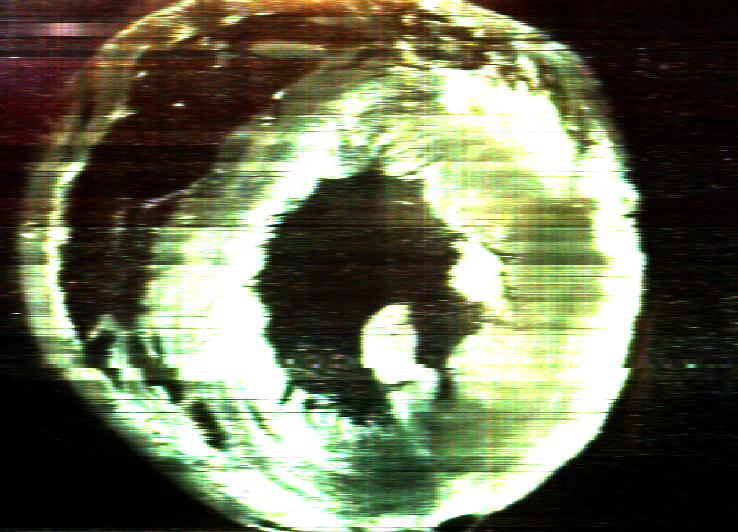
\includegraphics[height=1.2in]{3_results/Figs/LoRes_1_287}}
    \subfloat[]{
\includegraphics[height=1.2in]{3_results/Figs/geometric_1_287}}\\
    \subfloat[]{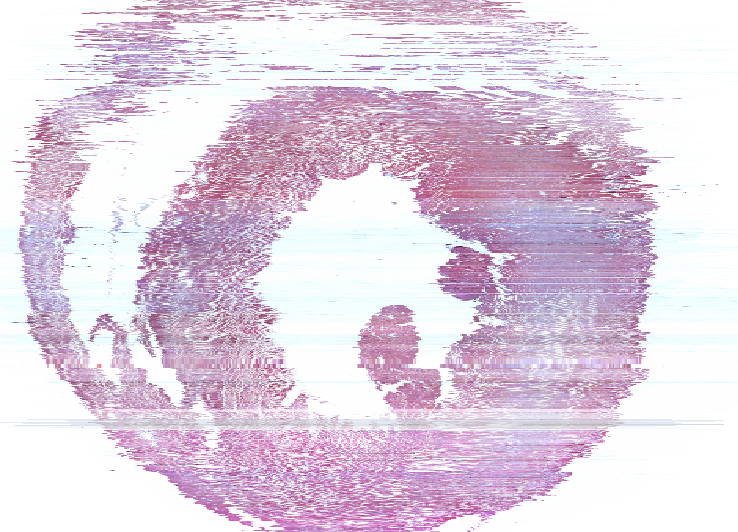
\includegraphics[height=1.2in]{3_results/Figs/affine_1_287}}
    \subfloat[]{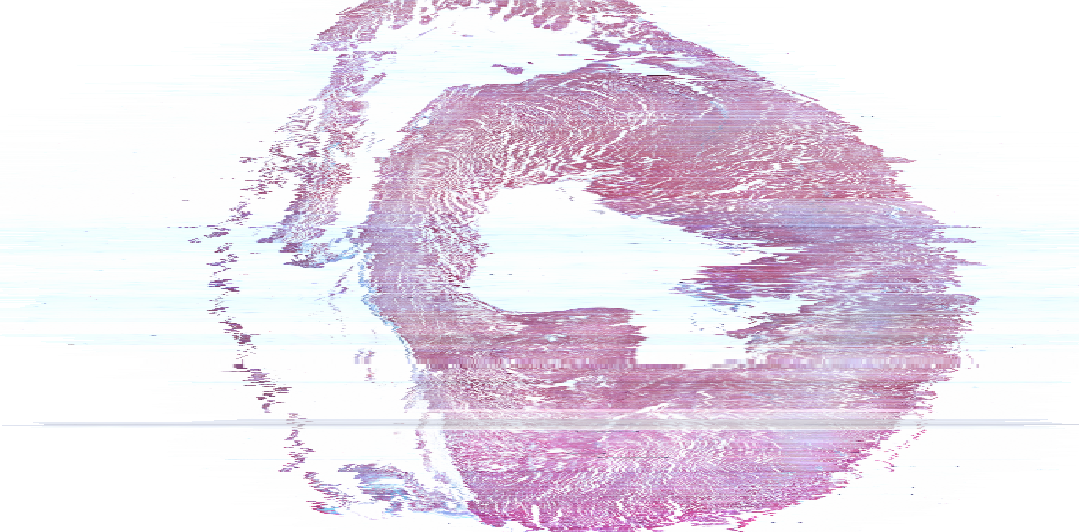
\includegraphics[height=1.2in]{3_results/Figs/banana_1_301}}
    \caption{Equivalent cross-sections of (a) the block face volume, (b) the histology slices before registration, aligned to their common geometrical centre, (c) the block face-registered histology slices and (d) the sequentially registered slices with no reference volume.}
    \label{fig:}
  \end{figure}
  
  Cross-sections of We achieve a reasonable large-scale alignment of the great majority of histological slices to form a consistent tissue volume. Yet we are left with several limitations of the block face technique. Striations are visible in (a) due to discrete changes in the positioning and intensity of illumination between block face image acquisitions. These changes will propagate to the final block face registration result. At 26.6 $\mu$m, the in-plane resolution of the reference images is 24 times coarser than that of the histology slices, precluding an alignment on the scale of cardiac microstructure. Small non-rigid deformations introduced during slicing and rehydration are particular to each slice, and could not be represented fully by the affine registration. Despite obtaining a result that was relatively close to the block face geometry, the overlap of pixel intensities between tissue and wax, and the interslice variability therein, led to a noisy, jagged result that was not always at the global minimum.
  
  MOVE TO RESULTS Even when constrained by a rigid transform, in many areas the slice-to-slice registration in (d) is accurate enough that detailed tissue structure is clearly visible. Yet, just as the cylinder does not represent the banana, the resulting geometry of the volume is quite unrelated to the ground truth of the block face volume. MOVE TO RESULTS
  
  FROM THESIS
  
  \subsection{Global Diffusion} % (fold)
  \label{sub:global_diffusion}
    % x slices
    \begin{figure}[htbp]
      \caption{Cross-sections of the full Rat28 volume perpendicular to the x-axis, after 0, 1 and 20 iterations of diffusion. The yellow boxes highlight the zoomed regions in Figure~\ref{fig:adjusted_bottom_vessels_0_235}.}
    \end{figure}

    % y slices
    \begin{figure}[htbp]
      \caption{Cross-sections of the full Rat28 volume perpendicular to the y-axis, after 0, 1 and 20 iterations of diffusion. The yellow boxes highlight the zoomed regions in Figure~\ref{fig:adjusted_bottom_vessels_1_287}.}
    \end{figure}
    
    20 iterations of smoothing were applied to the affine registered full-heart volume from Section~\ref{sec:registration_results}, and Figures~\labelcref{fig:adjusted_0_235,fig:adjusted_1_287} compare the central cross-sections of the volume before smoothing, after 1 iteration and after all 20 iterations. A subtle, but unmistakable improvement in coherence is observed; internal and external edges are smoother, especially towards the extremities of the heart, and clear, waving sheet structure has emerged, previously indistinguishable beyond the high-frequency zig-zagging noise.
    
    % lower 100 slices zoom
    % x slices
    \begin{figure}[htbp]
      \caption{Cross-sections of the lower 100 slices perpendicular to the x-axis. The blue arrows highlight blue-stained interstitial tissue around vessels, the green arrow epicardial vessels and the yellow arrow enhanced sheet structure.}
    \end{figure}

    % y slices
    \begin{figure}[htbp]
      \caption{Cross-sections of the lower 100 slices perpendicular to the y-axis. The green arrows highlight epicardial vessels and the yellow arrow enhanced sheet structure.}
    \end{figure}
    
    The effect is clearer in an enlargement of the bottom 100 slices in Figures~\labelcref{fig:adjusted_bottom_vessels_0_235,fig:adjusted_bottom_vessels_1_287}. The outer walls are several orders of magnitude less noisy in both figures, and internal vessel walls are much more coherent, most notably the epicardial vessels on the left and right of Figure~\ref{fig:adjusted_bottom_vessels_1_287}~(c). Sheet structure that started to surface from obscurity after just one iteration has been well resolved after 20 iterations. Figures~\labelcref{fig:whole_positive_x_diffused,fig:whole_negative_x_diffused,fig:whole_positive_y_diffused,fig:whole_positive_z_diffused} depict the smoother global contour after 20 iterations from several angles.
    
    % diffused contours
    \begin{figure}[p]
      \caption{Globally smoothed slice volume, viewed along the positive x direction.}
    \end{figure}

    \begin{figure}[p]
      \caption{Globally smoothed slice volume, viewed along the positive z direction.}
    \end{figure}
  % subsection global_diffusion (end)
  
  % subsection global_diffusion (end)
  
  \subsection{Regional Diffusion} % (fold)
  \label{sub:regional_diffusion}
      \begin{figure}[p]
        \caption{Central cross sections of the region around an epicardial vessel, perpendicular to the x axis. Cross-sections are compared before smoothing, after global smoothing and after smoothing applied to this region. The blue arrow highlights blue-stained interstitial tissue around vessels, the green arrow epicardial vessels and the yellow arrow enhanced sheet structure.}
      \end{figure}
    
      \begin{figure}[p]
        \caption{Central cross sections of the region around an epicardial vessel, perpendicular to the y axis.  The blue arrow highlights blue-stained interstitial tissue around vessels, the green arrow epicardial vessels and the yellow arrow enhanced sheet structure.}
      \end{figure}
    
      % \begin{figure}[p]
      %   \caption{Full resolution image of the central slice of the epicardial vessel region. The yellow box represents the bounds of Figure~\ref{fig:cropped_vessel_cross_section_z}.}
      % \end{figure}
      %     
      % \begin{figure}[p]
      %   \caption{A zoomed 200$\mu$m by 200$\mu$m square of full resolution image of the geometric centre of Figure~\ref{fig:vessel_cross_section_z}.}
      % \end{figure}
    
      A regional registration around an epicardial vessel yields even further improvement, when at this smaller scale, curvature and distortions not represented by an affine transformation become less significant. The final transforms from the global smoothings were used to initialise the regional smoothings, with the centre of transformation moved to the geometric centre of the region. In order to smooth the cost function adequately for the optimiser, the images used to perform the registration were Gaussian smoothed and downsampled by a factor of 8: a level optimal to resolve features the size of an epicardial vessel. Figures~\labelcref{fig:vessel_cross_section_x,fig:vessel_cross_section_y} show two central perpendicular cross-sections of the epicardial region before smoothing, after global smoothing and after an additional regional smoothing. Figures~\labelcref{fig:vessel_cross_section_z,fig:cropped_vessel_cross_section_z} remind us of the order-of-magnitude greater resolution in plane (1.1$\mu$m) with respect to the vertical out-of-plane resolution (10$\mu$m) in Figures~\labelcref{fig:vessel_cross_section_x,fig:vessel_cross_section_y}, displaying the central slice of the region at full resolution.
    
      \begin{figure}[p]
        \caption{Surface contours of segmentations of vasculature (red) and epicardium (green) in the region around an epicardial vessel from Figures~\labelcref{fig:vessel_cross_section_x,fig:vessel_cross_section_y,fig:vessel_cross_section_z,fig:cropped_vessel_cross_section_z}, from the unsmoothed, globally smoothed and locally smoothed volumes.}
      \end{figure}
    
       A confidence connected component segmentation was employed to generate the segmentations in Figure~\ref{fig:region_segmentations}, which, unlike methods such as level set segmentation or neighbourhood filters, does not introduce any artificial surface smoothing. Progressive enhancement in coherence is visible from the back cross-section, the vessel surface and the pericardial surface, from (a) to (b) and then to (c); the contours in (c) are almost totally smooth, with only the inherent stepping of each individual histology slice visible. In particular, the disturbance near the top of the largest vessel in (b) has been smoothed in (c). Original adjacent slice aberrations in (a) reached ~450$\mu$m. Contrastingly in (c), the relative registration error is reduced below the diameter of even the smallest vessels, by inspection less than 5$\mu$m in the large majority of cases - smaller than the width of a single myocyte. Resultingly, with each of the two smoothing procedures, more of the smaller vasculature has become connected to the main vessel and has been segmented.
    
      \begin{figure}[p]
        \caption{An overlay of the three vessel segmentations from Figure~\ref{fig:region_segmentations}. The unsmoothed vessel is shaded in red, the globally smoothed vessel in amber and the regionally smoothed vessel in green. }
      \end{figure}
    
      We see the combined results of all three vascular segmentations in Figure~\ref{fig:vessel_segmentations}. From this view through the pericardium, the striking continuity of the green surface is most apparent. The overall shape of the green vessel precisely intersects the disconnected set of red discs, demonstrating that the underlying vessel geometry has been recovered with remarkable accuracy. Again it is clear that the reduction in error below the diameter of the smallest vessels has facilitated their segmentation, with several thin green dendritic structures reaching up into the top left of the figure.
    
  % subsection regional_diffusion (end)
  
  FROM THESIS

  
  % figure of regional cross-section before smoothing, after global smoothing and after regional smoothing
  \begin{figure}[!t]
    \centering
    \subfloat[]{\includegraphics[width=3.4in]{3_results/Figs/unsmoothed_vessel_1_2125}}\\
    \subfloat[]{\includegraphics[width=3.4in]{3_results/Figs/globally_smoothed_vessel_1_2125}}\\
    \subfloat[]{\includegraphics[width=3.4in]{3_results/Figs/regionally_smoothed_vessel_1_2125}}
    \caption{}
    \label{fig:}
  \end{figure}
  
  % figure of vessel and surface contour before smoothing and after regional smoothing
  \begin{figure}[!t]
    \centering
    \subfloat[]{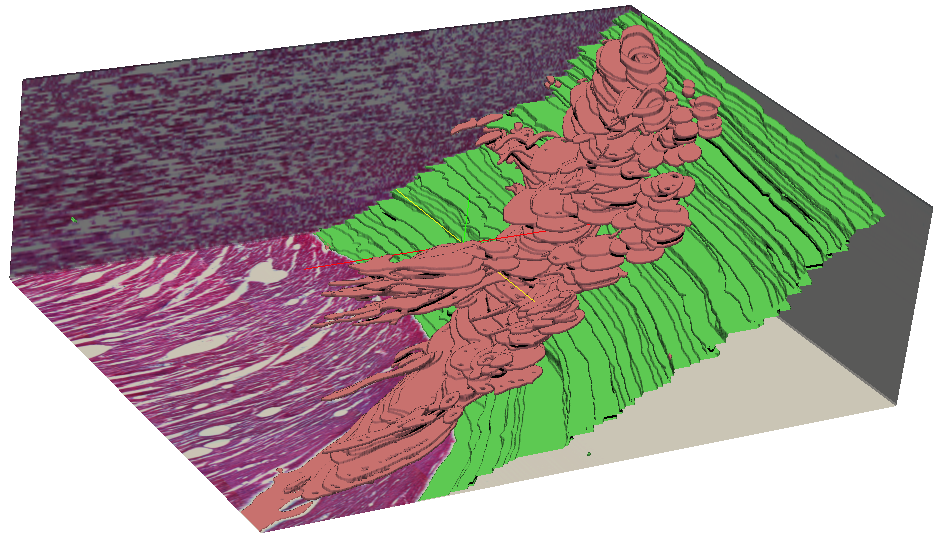
\includegraphics[width=3.4in]{3_results/Figs/unsmoothed_segmentation}}\\
    \subfloat[]{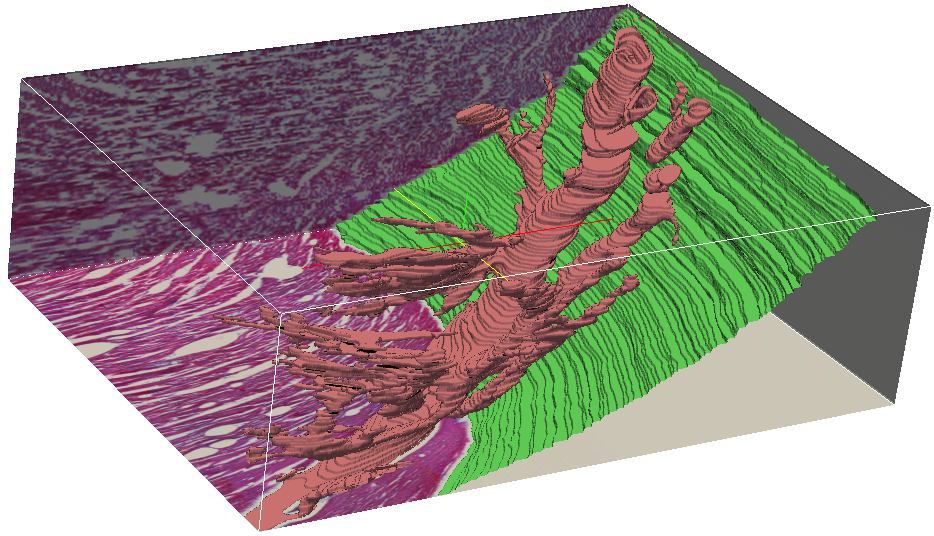
\includegraphics[width=3.4in]{3_results/Figs/globally_smoothed_segmentation}}\\
    \subfloat[]{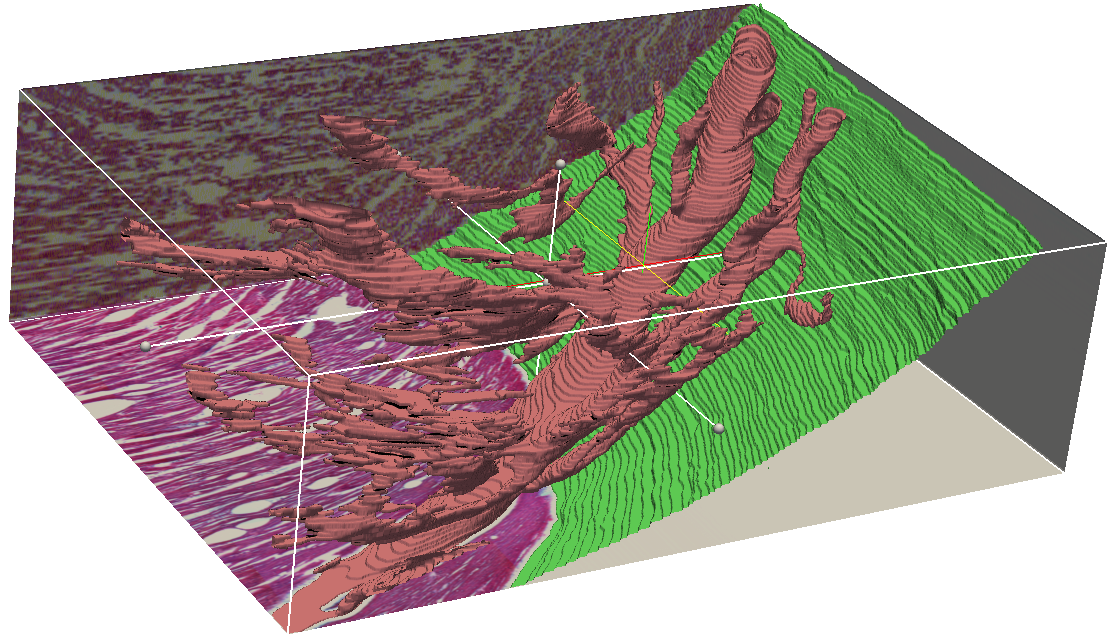
\includegraphics[width=3.4in]{3_results/Figs/locally_smoothed_segmentation}}
    \caption{}
    \label{fig:}
  \end{figure}
  
  % figure of vessel and surface contour before smoothing and after regional smoothing
  \begin{figure}[!t]
    \centering
    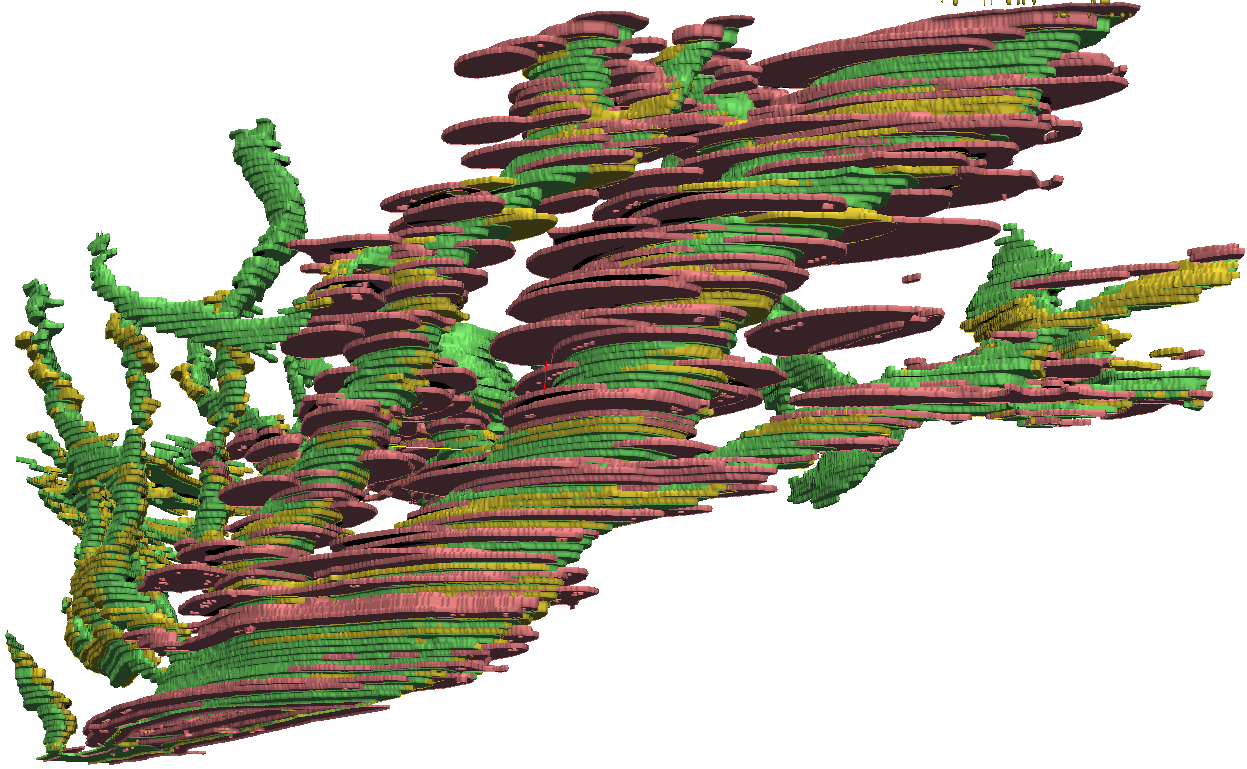
\includegraphics[width=3.4in]{3_results/Figs/vessel_overlay}
    \caption{}
    \label{fig:}
  \end{figure}
% section results (end)
